\subsection{Tracker}\label{tracker}

Accepts NoteProcessors: yes

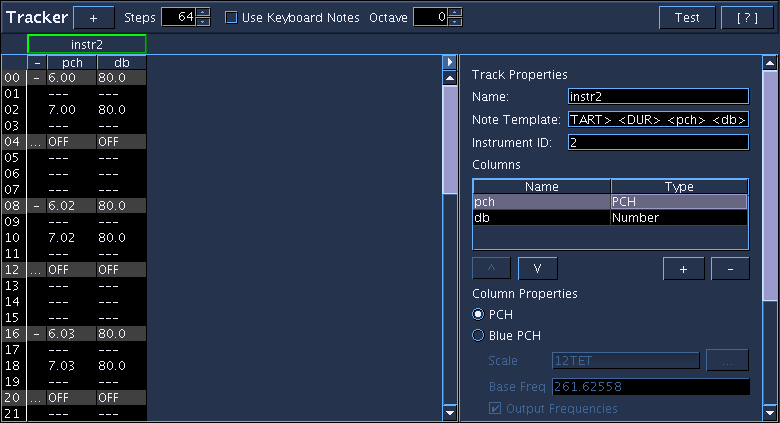
\includegraphics{images/tracker.png}

The Tracker SoundObject is a table-based tool to enter in patterns of
notes using the Tracker paradigm but in a way specific to Csound SCO
work. Each Tracker is organized in vertical Tracks of n number of steps
where n is configurable by the user (defaults to 64 steps). Notes are
entered into each Track with Tracks being configurable as to what
parameters (columns) to use. Unique to the blue Tracker SoundObject is
the support for microtonal scales using Scala scale files as well as
support for Csound's Tied-Notes feature.

The interface consists of three main areas: the top tool bar, the main
tracking area, and the track properties editor.

The top tool bar has a "+" button which adds new tracks to the Tracker,
a Steps entry widget to enter in the number of steps the Tracker should
have, a toggle for using Keyboard Note mode (see below for more
information), an Octave entry widget to determine the relative octave
for the Keyboard Note mode, a Test button to see what the generated
score will be for the Tracker, as well as a help button that opens up a
quick reference sheet for keyboard shortcuts.

The main tracking area is where all of the score work is done to enter
and modify notes. More information about note entry and modification is
available below in the section "Entering in Notes".

The last interface area is the track properties editor. The track
properties editor is held in a collapsible pane and when the tracker
editor initially loads it will be collapsed. To open up the track
properties, at least one track needs to be added to the tracker. Once
one track exists, click the small button above the right scroll bar to
open and close the track editor properties. More information on using
the properties editor follows below in the section "Settings Things Up".

When the Tracker Object is edited it is completely blank. To start,
click the "+" button to add as many tracks as you would like to use.
After adding the number of tracks you'd like to use you will need to
configure the track to work with your Csound instruments. Open up the
track properties editor using the "\textless{}" toggle button above the
right scroll bar. Afterwards, select a track by clicking the name panel
above a track. Selecting a track will populate the track properties
editor as well as hilight the name panel with a green border. A track's
properties consist of a Name, Note Template, Instrument ID, and Columns;
descriptions of the values are listed below.

\begin{description}
\item[Name]
The name property is used only for reference; editing the name changes
the title shown on the name panel and is for the user's reference.
\item[Note Template]
The note template is used when generating the notes for the track. Items
in the template that are within \textless{} and \textgreater{} tags will
be replaced by values either from the Tracker (START and DUR), the
Instrument ID (INSTR\_ID) or values from the columns, using the column's
name as a key (i.e. if a column is called "space", when generating a
note for the track, any value in the space column will replace the
\textless{}space\textgreater{} text in the note template). Note
templates will generally follow the form "i
\textless{}INSTR\_ID\textgreater{} \textless{}START\textgreater{}
\textless{}DUR\textgreater{}" and then have tag keys for each column for
the track.
\item[Instrument]
Instrument name or number to be used when replacing
\textless{}INSTR\_ID\textgreater{} in Note template strings.
\item[Columns]
Each track has a minimum of one configurable column (the tied-note is a
feature of all tracks and is not a part of this editor) and is
user-configurable to add as many columns as the user needs for the
values to use in their notes for their instruments. Columns are added
and removed using the Columns table and can be organized by pushing up
and down in the table which will move their order left and right in the
main tracking area. To edit the name of the Column, use the Columns
table to edit the name of the column.

Each Column also has a type. The type information is used by the tracker
when entering data to verify that the data being input is of that
column's type, as well as used when using shortcuts to manipulate data
in that column.

\begin{description}
\item[PCH]
Csound PCH format. Entering data will verify that data is in the
octave.pitch format. Using the increment and decrement value shortcuts
will propertly add or subtract one to pitch value, i.e. incrementing the
value of 8.11 will result in 9.00.
\item[blue PCH]
The blue PCH format is like the Csound PCH format except that the pitch
part is always a whole number integer and is the scale degree of the
selected Scale. A valid value in Csound PCH such as 8.01 is not valid in
Blue PCH as 01 is not an integer (the equivalent in blue PCH would be
8.1).

Using blue PCH allows for using Scala scale files to do microtonal
tracking. To choose a Scala scale, use the "..." button to open up a
file selector to choose a Scala scale. Afterwards, enter in the base
frequency for the scale (the default is 261.62558 or middle-c). The
"output frequencies" checkbox will determine how the values entered into
this column will be interpreted. By default, "output frequencies" is
enabled, meaning when the tracker goes to generate notes, it will take
the blue PCH values that are entered and convert them to a frequency
value in hertz. If you deselect this option, the tracker will pass the
blue PCH value out. This option should generally be left enabled unless
the user is planning to do further operation on the pch values via
NoteProcessors that work with blue PCH.

Using blue PCH, data will be verified on entry and increment/decrement
value options will work in the same way as for PCH.
\item[MIDI]
MIDI will limit the values entered to whole number integers from 0-127.
Using the increment and decrement value shortcuts will add or subtract 1
to the value.
\item[String]
The String type allows the user to input any value they want. No
verification is done on entry and the increment/decrement value
shortcuts will have no effect.
\item[Number]
The Number format will limit the values entered to only numbers. Values
can be further restricted to a given range as well as to only use whole
number integers. Using the increment and decrement value shortcuts will
add or subtract 1 to the value.
\end{description}
\end{description}

Entering in data into the tracker is much like entering data into any
other table, though learning the keyboard shortcuts will vastly speed up
entering and modifying data. To begin click anywhere on a track where
you would like to add a note. Now, begin typing to enter in a value for
that note, then press enter when you are finished. Depending on the type
of column you have configured, blue will verify that the data entered is
allowable and if so it will save that data to the note. If the value is
not allowable, the cell will become hilighted in red and will require
you to either fix your input to be valid or press esc to cancel entering
in data.

When entering in data for a new note, the first time you enter in
information for a column in the note's row, it will not only enter in
the data for the column, but also copy values for all other columns from
the first note that exists previous to the note being edited. If there
is no notes entered, some default settings will be used based on the
column type.

Like other tracker systems, the duration of a note entered will last as
long as until either the next entered note, the end of the pattern, or
until an OFF note is encountered. So, for example, if a note is entered
in step 0 and step 2, the duration of the first note will last 2 steps
while the second note will last until the end of the pattern (62 steps
in a default 64 step track). To enter an OFF statement, go to the row
where you want the note to end and press ctrl-shift-space. This will
make the row an OFF note. So, if a note is entered in step 0 and step 2
and an OFF is entered into step 1 and step 4, the first note will last 1
step while the second note will last 2 steps.

To increment and decrement values in a cell, use the arrow keys to go
over the cell you want to increment or decrement and then use ctrl-up or
ctrl-down respectively to change the value. (NOTE: This operation
operates differently for each column type and does nothing for the
String type. Please see the column type information above for more
information.)

Like most trackers, the Tracker object has keyboard shortcuts that will
allow for very quickly adding notes. To enable Keybaord Note mode,
either click the checkbox on the top tool bar or use the keyboard
shortcut ctrl-k. By enabling Keyboard Note mode, the keys on the
keyboard will be mapped to note values much like a piano keyboard. When
the selected cell is of type PCH, blue PCH, or MIDI, pressing those keys
will enter in a value related the keyboard mapping (see Shortcuts
section).

The user is also able to change the base octave of the Keyboard Note
mode. To change the octave, use either the spinner control on the top
tool bar or use the keyboard shortcuts ctrl-shift-up or ctrl-shift-down.
By default, the base octave starts at middle-c.

\begin{longtable}[]{@{}ll@{}}
\caption{Keyboard Shortcuts}\tabularnewline
\toprule
Shortcuts & Description\tabularnewline
\midrule
\endfirsthead
\toprule
Shortcuts & Description\tabularnewline
\midrule
\endhead
ctrl-space & clear or duplicate previous note\tabularnewline
ctrl-shift-space & set or clear OFF note\tabularnewline
ctrl-up & increment value\tabularnewline
ctrl-down & decrement value\tabularnewline
ctrl-t & toggle note tie\tabularnewline
ctrl-x & cut selected notes\tabularnewline
ctrl-c & copy selected notes\tabularnewline
ctrl-v & paste notes from copy buffer\tabularnewline
insert & insert blank note into currently selected row, notes in current
row and after are shifted down; if notes are at end are shifted off they
are lost\tabularnewline
del & delete selected note(s), move selection to next row after current
selection\tabularnewline
shift-backspace & delete selected notes, notes after selected notes are
shifted up to fill in place where deleted notes were, empty notes
appended to end\tabularnewline
ctrl-k & toggle keyboard notes mode\tabularnewline
ctrl-shift-up & raise keyboard octave by one\tabularnewline
ctrl-shift-down & lower keyboard octave by one\tabularnewline
\bottomrule
\end{longtable}

\begin{longtable}[]{@{}llll@{}}
\caption{Keyboard Note Mode}\tabularnewline
\toprule
Shortcut & PCh Value & blue PCH Value & MIDI Value\tabularnewline
\midrule
\endfirsthead
\toprule
Shortcut & PCh Value & blue PCH Value & MIDI Value\tabularnewline
\midrule
\endhead
z & 8.00 & 8.0 & 60\tabularnewline
s & 8.01 & 8.1 & 61\tabularnewline
x & 8.02 & 8.2 & 62\tabularnewline
d & 8.03 & 8.3 & 63\tabularnewline
c & 8.04 & 8.4 & 64\tabularnewline
v & 8.05 & 8.5 & 65\tabularnewline
g & 8.06 & 8.6 & 66\tabularnewline
b & 8.07 & 8.7 & 67\tabularnewline
h & 8.08 & 8.8 & 68\tabularnewline
n & 8.09 & 8.9 & 69\tabularnewline
j & 8.10 & 8.10 & 70\tabularnewline
m & 8.11 & 8.11 & 71\tabularnewline
q & 9.00 & 9.0 & 72\tabularnewline
2 & 9.01 & 9.1 & 73\tabularnewline
w & 9.02 & 9.2 & 74\tabularnewline
3 & 9.03 & 9.3 & 75\tabularnewline
e & 9.04 & 9.4 & 76\tabularnewline
r & 9.05 & 9.5 & 77\tabularnewline
5 & 9.06 & 9.6 & 78\tabularnewline
t & 9.07 & 9.7 & 79\tabularnewline
6 & 9.08 & 9.8 & 80\tabularnewline
y & 9.09 & 9.9 & 81\tabularnewline
7 & 9.10 & 9.10 & 82\tabularnewline
u & 9.11 & 9.11 & 83\tabularnewline
i & 10.00 & 10.0 & 84\tabularnewline
9 & 10.01 & 10.1 & 85\tabularnewline
o & 10.02 & 10.2 & 86\tabularnewline
0 & 10.03 & 10.3 & 87\tabularnewline
p & 10.04 & 10.4 & 88\tabularnewline
\bottomrule
\end{longtable}

\begin{quote}
\textbf{Note}

See the tracker.blue example file in the blue/examples/soundObjects
folder.
\end{quote}
